\NextFile{GTFS2TransitSchedule.html}
\section{GTFS2TransitSchedule}

This guide whill show you how to convert GTFS data to a MATSim Transit Schedule

\subsubsection{Automatic conversion}
\begin{itemize}
	\item Put the set of GTFS files of each public transport system in a different folder of your file system.
	\item Create a java program that constructs an object of the class
\texttt{GGTFS2MATSimTransitSchedule}in the package 
\texttt{GTFS2PTSchedule} which is part of this extension.For this you need to specify:
\end{itemize}
\begin{enumerate}
	\item An array of folders (
\texttt{File} class) where your public transport system specifications are located.
	\item An array of Strings representing the network modes correspondent to each public transport defined in b) (e. g. “
\texttt{car}” for buses, “
\texttt{rail}” for metro).
	\item The MATSim network object with the nodes in latitude and longitude coordinates (
\texttt{WGS84}).
	\item An array of Strings with the names of the calendar services that are desired (e. g. “
\texttt{weekday}”, “
\texttt{daily}”). Remember that MATSim only simulates one day, but the GTFS files specify routes for many calendar days or dates.
	\item The desired output coordinates system
\end{enumerate}
\begin{itemize}
	\item Call the method 
\texttt{TransitSchedule getTransitSchedule()}.  Then, each route of each given public transit systems will be processed  with the semi-automatic procedure presented in the following figure.
\end{itemize}
\begin{figure}[htp]
	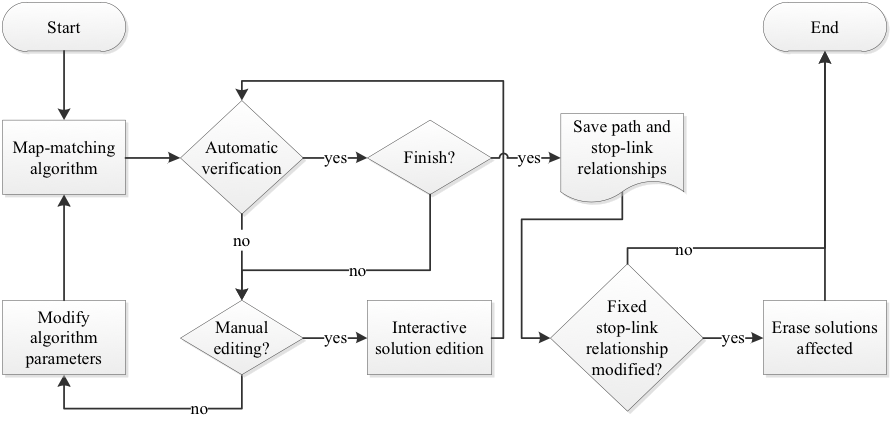
\includegraphics{figures/gtfs2schedule/gtfsAutoConversion.png}
\end{figure}




\subsubsection{Manual correction of automatic conversion}

For the manual editing process one can visualize, edit and verify the solution for each route:
\begin{itemize}
	\item Visualization: A navigation network is displayed, including all  relevant information for working with one single route. This includes  the route’s profile, the given sequence of GPS points and its current  solution (path and stop-link relationships). Selected elements are drawn  in a different color. All is displayed in a bi-dimensional interactive  way with refresh of the cursor location in the working coordinates, and  panning,  zoom and view-all options.
	\item Selection: Different options for selecting elements of the solution  or elements from the network are provided. It is possible to select the  nearest link (solution or network), nearest node (network) or nearest  stop (solution) to a point indicated by the user. When a stop that has a  stop-link relationship already, the corresponding link is selected as  well. If a link of the solution path is selected and it does not have a  subsequent link connected, a new one from the network is selected with  one click; the selected link is the one with the most similar angle than  the line defined by the end node of the initial link and a point  indicated by the user.
	\item Solution modification: The first link of the sequence can be added  selecting any link of the network. If a link of the solution path does  not have a subsequent link connected, it is possible to add one  according to the selection function described in (b). If there are two  subsequent links in the solution that are not connected (a gap), a  subsequence that connects the mentioned links is added, using the  shortest path algorithm, with the current parameters. Furthermore,  selecting one link of the path, it is possible to delete it, or to  delete all the links before or after it. Finally, stop-link  relationships can be modified selecting both elements. If the modified  relationship was fixed, the user  is prevented because the tool erase  the solutions of the routes to which the selected stop belongs.
	\item Network modification: New nodes to the road network can be added. In  addition, with any node selected, it is possible to add a new link  selecting the end node.
\end{itemize}

Hints and interaction details:
\begin{itemize}
	\item It is necessary to pass the verification process (“Is OK”) for saving a route result
	\item The routes are saved in temporal files located in the ./data/paths/ folder relative to the program location.
	\item Panning and zoom functions are provided dragging the mouse and moving the mouse wheel.
	\item View all function is provided typing the “v” key
	\item Up and down keys allow to select the next or previous link of the path.
	\item “$<$” or ”$>$” keys allow to select the previous or next stop 

\begin{figure}[htp]

\end{figure}
	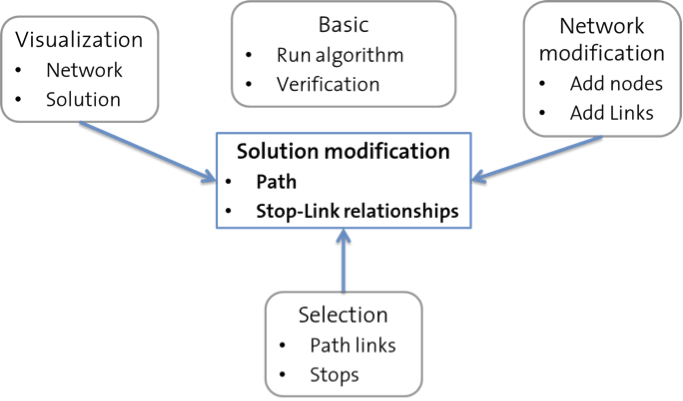
\includegraphics{figures/gtfs2schedule/gtfsManualEdit.png}
\end{itemize}

\subsubsection{Saving the converted data}

Finally, after the semi-automatic process, the Transit Schedule  object is returned and the network object is modified (splitting, new  nodes and links, and modes of the links). One can save in a XML  the 
\texttt{TransitSchedule} object constructing a 
\texttt{TransitScheduleWriter} object, and the modified network with a 
\texttt{NetworkWriter}.
